\documentclass{article}
\usepackage{blindtext}
\usepackage{graphicx}
\usepackage[utf8]{inputenc}
\usepackage{graphicx}
\usepackage{natbib}
\usepackage{float}
\usepackage{amsmath}
\usepackage{siunitx}
\usepackage{indentfirst}

\title{Trabalho Prático I: Biblioteca de Threads Compact Threads (cthreads)}
\author{Cristiano Salla Lunardi - 240508 \cr
Gustavo Madeira Santana - 252853 \cr\cr
INF01142 - Sistemas Operacionais I N - 2016/2\cr\cr
Prof. Alexandre Carissimi}
\date{}

\begin{document}

\maketitle

\section{Introdução}
Este relatório tem como objetivo descrever o que foi desenvolvido no primeiro trabalho prático da disciplina (INF01142) Sistemas Operacionais I N. A proposta desse trabalho é desenvolver uma biblioteca de threads \textit{Compact Threads}, ou \textit{cthreads}, para manipular threads em execução em um sistema operacional.

O desenvolvimento foi feito na linguagem C e usando uma máquina virtual em ambiente GNU/LINUX.

\begin{figure}[b]
    \centering
    \includegraphics[scale=0.4]{imagens/DiagramaDeEstados.png}
    \caption{Diagrama de estados da biblioteca \textit{cthreads}}
    \label{fig:sym4}
\end{figure}

\section{Biblioteca \textit{Compact Threads}}
A biblioteca, implementada fundamentalmente no arquivo \textit{cthread.c}, possui todas funções requeridas para manipular as threads \footnotemark, também possuí funções auxiliares como a função\textit{cscheduler} que faz o sorteio da thread que entrará em execução e a função \textit{init\_cthreads}, que cuida da inicialização das estruturas de dados usadas pela biblioteca, bem como inicialização do scheduler e da thread para a função main.
\footnotetext{ccreate, cyield, cjoin, csem\_init, cwait, csignal}

O funcionamento de cada função será destacado nas seções seguintes.

\subsection{Função \textit{ccreate}}
Principal função da biblioteca, \textit{ccreate} é usada para criar threads e associa-lá a uma função. Recebe como parâmetros uma função e um argumento e retorna o \textit{tid} da thread criada.

\begin{figure}[h]
    \centering
    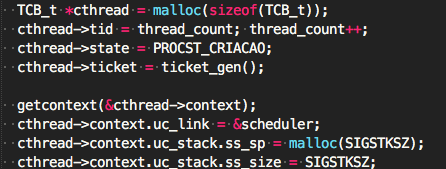
\includegraphics[scale=0.4]{imagens/ccreate.png}
    \caption{Criação e definição do contexto de uma nova thread}
    \label{fig:sym4}
\end{figure}

Para criação da thread, é realizado uma alocação na memória para o \textit{TCB}, e alguns dados são inicializados. A thread receberá uma \textit{tid}, valor inteiro que é incrementado a cada criação. Seu estado durante a criação é 0\footnotemark. Para criar o contexto da thread, inicialmente é feito uso da função \textit{getcontext} para ter o modelo pronto, depois então é definido que ao fim da execução da thread, o contexto a ser carregado deve ser o do \textit{scheduler}, através do \textit{uc\_link}. Também é feita uma alocação de memória para a pilha que será usada pelo contexto, através da \textit{ss\_sp} e \textit{ss\_size}.
\footnotetext{\textit{PROCST\_CRIACAO}}

Por fim,  ao ser inserido na fila de aptos, seu estado é alterado para 1\footnotemark e a criação está completa.
\footnotetext{\textit{PROCST\_APTO}}

\subsection{Função \textit{cyield}}
Para "passar a vez" voluntariamente, onde a thread retorna para a fila de aptos após ceder voluntariamente sua vez na execução.

A thread que chamou a função \textit{cyield} tem seu estado alterado para \textit{PROCST\_APTO} e inserido de volta na fila de aptos. O controle é então passado para o \textit{scheduler}.

\subsection{Função \textit{cjoin}}
Usada para bloquear uma thread até que outra thread termine sua execução. Tem como único parâmetro o valor do \textit{tid} da thread que deverá finalizar sua execução.
A função que chamou \textit{cjoin} só voltará para a fila de aptos após a thread indicada terminar.

Foi criado uma estrutura auxiliar chamada de \textit{Join Control Block}, ou \textit{JCB}. Neste descritor é armazenado qual thread será bloqueada, e o \textit{tid} da thread que a libera. Existe ainda uma função auxiliar \textit{cunjoin\_thread} que cuida do desbloqueio da thread quando a indicada termina sua execução, seu comportamento é descrito em outra seção.

\begin{figure}[ht]
    \centering
    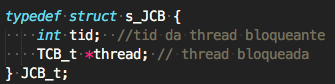
\includegraphics[scale=0.4]{imagens/jcb.png}
    \caption{Join Control Block, descritor auxiliar para controlar threads com \textit{join}}
    \label{fig:sym4}
\end{figure}

\subsection{Função \textit{csem\_init}}
Nesta função é inicializado o \textit{semáforo}. Recebe como parâmetros um ponteiro para a struct do semáforo e a quantidade de recursos que este semáforo terá. Para simular um \textit{mutex}, a quantidade de recursos deve ser \textit{1}.

Para inicializar o semáforo é criado uma fila, onde será armazenado quais threads estão disputando recursos. Para usar ou liberar um recurso, são usadas as funções \textit{cwait} e \textit{signal}, respectivamente. Seus comportamentos são explicados a seguir

\subsection{Função \textit{cwait}}
A função \textit{cwait} tem como finalidade fazer a requisição de recursos do \textit{semáforo}. Caso o semáforo tenha recursos disponíveis, seu indicador de recursos é decrementado e a thread segue sua execução. Caso não haja recursos disponíveis, a thread é bloqueada e entra para a fila do semáforo.

\subsection{Função \textit{csignal}}
A função \textit{csignal} é usada para indicar que a thread está liberando recursos para o semáforo. Uma vez que ela é chamada, o número de recursos do semáforo é incrementado, consequentemente a primeira thread na fila do semáforo é colocada na fila de aptos, podendo então fazer uso do recurso liberado pela thread que chamou a função \textit{csignal}.

\section{Funções Auxiliares}

\subsection{Função \textit{init\_cthreads}}
Essa função tem a finalidade de inicializar as estruturas de dados usadas pela biblioteca, bem como inicialização do contexto do \textit{scheduler} e da thread para a função \textit{main}. Nele são inicilizadas filas para as threads que estão em estado \textit{Apto} e \textit{Bloqueado}, e também do ponteiro para a thread que está em execução, que ao inicializar é a \textit{main}.

\subsection{Função \textit{cscheduler}}
O \textit{scheduler} implementado é do tipo não preemptivo, sem priodidades, e segue uma política de loteria. Toda thread ao ser criada recebe um bilhete \footnotemark, número aleatório entre 0 e 255. O \textit{scheduler} então sorteia um número e escolhe a thread que tem um bilhete mais próximo do sorteado. Em caso de duas threads com mesmo bilhete, a escolhida será a  que tiver menor \textit{tid}.
\footnotetext{o número é gerado pela função ticket\_gen}

\begin{figure}[h]
    \centering
    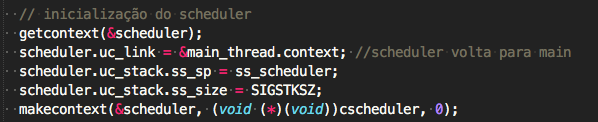
\includegraphics[scale=0.4]{imagens/scheduler.png}
    \caption{Inicialização do scheduler, e criação de seu contexto}
    \label{fig:sym4}
\end{figure}

\subsection{Função \textit{find\_thread}}
Função auxiliar para saber se uma dada thread existe em uma dada fila. Recebe como parâmetros um \textit{tid} e uma \textit{fila} (fila de aptos ou bloqueados por exemplo). Retorna \textit{0} se a thread foi encontrada ou \textit{-1} se a thread não foi encontrada.

\subsection{Função \textit{remove\_thread}}
Função auxiliar para remover uma dada thread em uma dada fila. Recebe como parâmetros um \textit{tid} e uma \textit{fila} (fila de aptos ou bloqueados por exemplo). Retorna \textit{0} se a thread foi encontrada e removida ou \textit{-1} se não foi possível remover a thread especificada.

\subsection{Função \textit{cunjoin\_thread}}
Esta função foi criada para auxiliar a função \textit{cjoin}. Toda vez que o \textit{scheduler} entra em execução, a função \textit{cunjoin\_thread} é chamada para verificar se a thread que acabou de terminar sua execução estava segurando alguma outra thread \footnotemark. Em caso positivo, a função remove esta interdepedência de threads e coloca a thread bloqueada na fila de \textit{aptos}.
\footnotetext{através do uso da função cjoin}

\subsection{Função \textit{ticket\_gen}}
Encarregada de gerar um número aleatório entre \textit{0} e \textit{255}, para ser usada como bilhete da thread, assim como número sorteado no processo de escolha de uma thread pelo \textit{scheduler}. Faz isso da função \textit{Random2} fornecida pelo arquivo \textit{support.o}.

\subsection{Função \textit{cidentify}}
Ao chamar esta função, é mostrado os componentes do grupo.

\subsection{Funções \textit{debugOn} e \textit{debugOff}}
Função auxiliar para fazer o debug da biblioteca. Ao chamar \textit{debugOn}, diversos \textit{printf} são ativados nas funções para ficar evidente ao usuário o que está sendo feito. Para desativar basta chamar a função \textit{debugOff}. Ambas não recebem nenhum parâmetro.

\section{Testes}

Todos testes podem ser executados com o modo debug ligado, basta adicionar debug ao nome do teste. Por exemplo, para o teste1 seria executado ./teste1debug em favor de ./teste1. Para o teste2 se executaria ./teste2debug, e assim por diante.

\subsection{Teste do \textit{ccreate} com \textit{cyield}}
\begin{itemize}
\item Arquivo: teste1.c | ./teste1 | ./teste1debug
\item Funções usadas: ccreate, cyield
\item Threads criadas: 104
\end{itemize}

\subsection{Teste do \textit{cjoin}}
\begin{itemize}
\item Arquivo: teste2.c | ./teste2 | ./teste2debug
\item Funções usadas: ccreate, cjoin, cyield
\item Threads criadas: 3
\end{itemize}

\subsection{Teste do \textit{semáforo}}
\begin{itemize}
\item Arquivo: teste3.c | ./teste3 | ./teste3debug
\item Funções usadas: ccreate, csem\_init, cwait, csignal, cyield
\item Threads criadas: 5
\end{itemize}

\section{Problemas}
\subsection{Segmentation fault...}
Um problema foi identificado ao misturar a função cjoin com as diretivas do semáforo. Dependendo da ordem que ocorre a execução, por exemplo, cwait seguindo de um cjoin, o teste é encerrado com erro de segmentação.

Um dos comandos usados para debug foi:
\begin{verbatim}
valgrind --trace-children=yes --track-fds=yes --log-fd=2
--error-limit=no --leak-check=full --show-possibly-lost=yes
--track-origins=yes --show-reachable=yes <executavel>
\end{verbatim}

Diversos erros de segmentação foram corrigodos durante a produção do trabalho. Alocações estáticas foram trocadas por alocações dinâmicas onde era conveniente. Também foi implementado um melhor controle do que não estava mais em uso, consequentemente liberando a memória e evitando então erros de segmentação. O único erro que restou foi o que envolve o cjoin em uso com o operador de semáforo.

\end{document}